\documentclass[11pt,a4paper]{article}

% ── Packages ──────────────────────────────────────────────────────────────────
\usepackage[T1]{fontenc}
\usepackage[utf8]{inputenc}
\usepackage{lmodern}
\usepackage[margin=2.5cm]{geometry}
\usepackage{amsmath,amssymb,amsthm}
\usepackage{booktabs}
\usepackage{array}
\usepackage{graphicx}
\usepackage[labelfont=bf,font=small,skip=4pt]{caption}
\usepackage{subcaption}
\usepackage{float}
\usepackage{xcolor}
\usepackage[colorlinks=true,linkcolor=blue!60!black,citecolor=green!50!black,
            urlcolor=blue!70!black]{hyperref}
\usepackage{microtype}
\usepackage{parskip}
\usepackage{enumitem}
\usepackage{fancyhdr}

% ── Page style ────────────────────────────────────────────────────────────────
\pagestyle{fancy}
\fancyhf{}
\rhead{\small ERF Study (Task 5)}
\lhead{\small G.\,Scriven}
\cfoot{\thepage}
\renewcommand{\headrulewidth}{0.4pt}

% ── Convenience macros ────────────────────────────────────────────────────────
\newcommand{\eps}{\varepsilon}
\newcommand{\thd}{\theta_d}
\newcommand{\sres}{\sigma_{\mathrm{res}}}
\newcommand{\sscat}{\sigma_{\mathrm{scatt}}}
\newcommand{\ntrk}{T}
\newcommand{\Nseg}{N_{\mathrm{seg}}}
\newcommand{\cosQC}{\cos\theta_{QC}}
\newcommand{\codepath}[1]{\texttt{#1}}

% Abstract box with shaded background
\newsavebox{\abstractsavebox}
\newenvironment{abstractbox}{%
  \setlength{\fboxsep}{8pt}%
  \begin{lrbox}{\abstractsavebox}%
  \begin{minipage}{0.86\linewidth}%
  \textbf{Abstract}\par\smallskip
}{%
  \end{minipage}%
  \end{lrbox}%
  \begin{center}\colorbox{gray!10}{\usebox{\abstractsavebox}}\end{center}%
}

% ── Title ─────────────────────────────────────────────────────────────────────
\title{%
  \textbf{ERF Study (Task 5)}\\[4pt]
  \large The Smooth (\texttt{erf}) Angular-Cost Hamiltonian for the
  TrackHHL Segment-Level Algorithm\\[2pt]
  \normalsize Toy LHCb VELO Characterisation Study}
\author{G.\,Scriven\\[2pt]
  \small Nikhef / Maastricht University / Hasselt University}
\date{June 2026}

% ══════════════════════════════════════════════════════════════════════════════
\begin{document}
\maketitle
\thispagestyle{fancy}

% ── Abstract ──────────────────────────────────────────────────────────────────
\begin{abstractbox}
This report characterises a \emph{smooth} angular-compatibility cost for the TrackHHL
1-Bit Quantum Filter (1BQF)~\cite{onebqf} segment-level Hamiltonian, replacing the hard
step-function acceptance with the error-function (\texttt{erf}) kernel
$C(\theta)=1+\mathrm{erf}\!\big((\eps-\theta)/(\thd\sqrt2)\big)$, whose width $\thd$ is a
tunable smoothing scale. On a fixed reference event ($\ntrk=50$ tracks, five planes) we
compare the step and \texttt{erf} Hamiltonians side by side: their matrix structure and
eigenspectra, their classical and quantum solution vectors, and their segment-level
efficiency / purity. Four findings are reported.
\begin{enumerate}[noitemsep,topsep=2pt]
  \item At the validated absolute operating threshold ($x>0.35$), the step function is
        \emph{already perfect} in low noise (efficiency $=1.00$, false rate $=0.00$); the
        \texttt{erf} kernel matches it but adds a small false-rate penalty
        ($\le 2\%$) by giving partial weight to borderline-false pairs.
  \item The \texttt{erf} kernel's advantage is \emph{robustness to measurement
        resolution}: at $\sres=0.02\,\mathrm{mm}$ the step efficiency collapses to
        $0.46$--$0.53$ while \texttt{erf} ($\thd=10^{-3}$) recovers it to $0.76$--$0.80$,
        a $+0.27$ to $+0.34$ absolute gain.
  \item The \texttt{erf} kernel roughly \emph{doubles the quantum fidelity}: at
        $\ntrk=10$ the cosine between the 1BQF and classical solutions rises from
        $\cosQC=0.47$ (step) to $0.84$ (\texttt{erf}, $\thd=10^{-4}$), despite a larger
        matrix condition number.
  \item The smoothing is noise-invariant in spectrum: the condition number
        $\kappa$ depends only on $\thd$ ($\kappa_{\rm step}=2.4$,
        $\kappa_{\rm erf}=8.6$--$9.5$) and is unchanged by hit drop.
\end{enumerate}
This is the local, single-event portion of the study; the full HTCondor sweep over
$\thd\times(\sscat,\sres)\times\ntrk$ (882 jobs) is in progress and will extend the
quantitative landscape.
\end{abstractbox}

\tableofcontents
\newpage

% ══════════════════════════════════════════════════════════════════════════════
\section{Introduction}
\label{sec:intro}

The TrackHHL segment-level algorithm~\cite{onebqf} reconstructs trajectories by solving
the linear system $A\mathbf{x}=\mathbf{b}$, where each $x_i$ is the activation of a
hit-to-hit \emph{segment} and the compatibility matrix $A$ couples two segments sharing a
middle hit when their kink angle $\theta$ is small. All previous tasks in this series use
a \emph{hard} acceptance: a triplet contributes a coupling of $1$ if $\theta<\eps$ and $0$
otherwise. This report (Task~5) studies the only variant with a \emph{soft} acceptance,
in which the binary cut is replaced by a smooth \texttt{erf} kernel of tunable width
$\thd$. The step function is recovered as $\thd\to0$, which doubles as a regression check.

The motivation is twofold. Physically, a soft kernel weights triplets by how compatible
they are rather than accepting or rejecting them outright, which could improve tolerance
to measurement smearing near the acceptance boundary. Algorithmically, the smoothing
reshapes the spectrum of $A$, which directly affects the quantum (HHL) solver whose cost
and fidelity depend on the eigenvalue distribution.

Section~\ref{sec:theory} defines both Hamiltonians and the scoring convention.
Section~\ref{sec:design} describes the fixed reference event and the parameter grid.
Section~\ref{sec:results} presents the structural, solution-vector, segment-metric, and
quantum comparisons. Sections~\ref{sec:discussion}--\ref{sec:conclusions} interpret the
results and state conclusions.

% ══════════════════════════════════════════════════════════════════════════════
\section{Theoretical Framework}
\label{sec:theory}

\subsection{The step and \texttt{erf} Hamiltonians}
A triplet is two segments sharing a middle hit on consecutive planes, with kink angle
$\theta=\arccos(\hat v_{\rm in}\!\cdot\!\hat v_{\rm out})$. The two compatibility kernels
are
\begin{align}
  C_{\rm step}(\theta) &= \begin{cases} 1 & \theta<\eps \\ 0 & \text{otherwise} \end{cases},
  &
  C_{\rm erf}(\theta) &= 1 + \mathrm{erf}\!\left(\frac{\eps-\theta}{\thd\sqrt2}\right).
\end{align}
$C_{\rm erf}$ is a smooth sigmoid in $[0,2]$ centred on $\theta=\eps$ with transition
width set by $\thd$. As $\thd\to0$ it approaches $2\,C_{\rm step}$; for finite $\thd$ it
assigns partial weight to triplets near the boundary. The off-diagonal entries of $A$ are
$-C(\theta)$ (attractive coupling), and the diagonal is the constant $\gamma+\delta=4$
(with $\gamma=3,\delta=1$), independent of the kernel. The right-hand side is
$\mathbf{b}=\delta\mathbf{1}$.

\subsection{Matrix density}
For the clean reference event ($\ntrk=50$, $\Nseg=10\,000$) the step matrix has
$\mathrm{nnz}=10\,300$ (essentially diagonal plus the $\sim\!150$ true triplet couplings),
whereas every \texttt{erf} matrix has $\mathrm{nnz}=760\,000$ --- about $74\times$ denser
--- because all mid-hit pairs receive a (possibly tiny) non-zero weight. The \texttt{erf}
kernel therefore trades sparsity for smoothness (Fig.~\ref{fig:structure}).

\subsection{The scoring convention}
\label{sec:theory:thresh}
Segment metrics are evaluated by thresholding the solution vector at the
\emph{absolute} value $x>0.35$, the validated convention from the segment-level
baseline (\codepath{Verify\_new\_results/segment\_level\_analysis.ipynb}). Its
justification is the Hopfield fixed-point structure of $A$: an isolated/false segment
relaxes to $\delta/(\delta+\gamma)=0.25$, while a true segment in a compatible chain sits
on a $\approx0.375$ plateau, so $0.35$ separates the two populations. A \emph{relative}
threshold $\tau\cdot\max(x)$ must \emph{not} be used: it collapses below both levels and
produces a spurious false rate near unity.

% ══════════════════════════════════════════════════════════════════════════════
\section{Study Design}
\label{sec:design}

The reference event is $\ntrk=50$ pion tracks on five planes
($\Delta z=33\,\mathrm{mm}$, $z_0=33\,\mathrm{mm}$, $\pm40\,\mathrm{mm}$ active area,
cone $|\phi|,|\theta|\le0.2$), generated with a fixed seed so that the step and
\texttt{erf} Hamiltonians see identical hits. The smoothing width is swept over
$\thd\in\{10^{-6},10^{-5},5\!\times\!10^{-5},10^{-4},5\!\times\!10^{-4},10^{-3}\}$, with
$\thd=10^{-6}$ serving as the step-function regression point. Three experimental sections
are reported: (i)~a perfectly clean event ($\sscat=\sres=0$, no hit drop); (ii)~the same
event with a $1\%$ hit-drop noise; and (iii)~a scan over
$\sscat\in\{0,10^{-4},5\!\times\!10^{-4}\}$ and
$\sres\in\{0,5\!\times\!10^{-6},0.02\}\,\mathrm{mm}$. Eigenspectra are computed on a
smaller $\ntrk=20$ event (dense \texttt{eigvalsh}); the quantum comparison uses
$\ntrk=10$ ($\Nseg=400$, 9~system qubits) on a CPU statevector simulator. All segment
construction and metrics use the optimised \codepath{SimpleHamiltonianFast} and Numba
\codepath{fast\_segment\_metrics} code paths. The full multiplicity landscape
($\thd\times$ noise $\times\,\ntrk$ up to $1000$, quantum for $\ntrk\le200$) is being
produced on HTCondor and is not yet included here.

% ══════════════════════════════════════════════════════════════════════════════
\section{Results}
\label{sec:results}

\subsection{Hamiltonian structure and eigenspectrum}
\label{sec:results:struct}

\begin{figure}[H]
  \centering
  \begin{subfigure}{0.48\linewidth}
    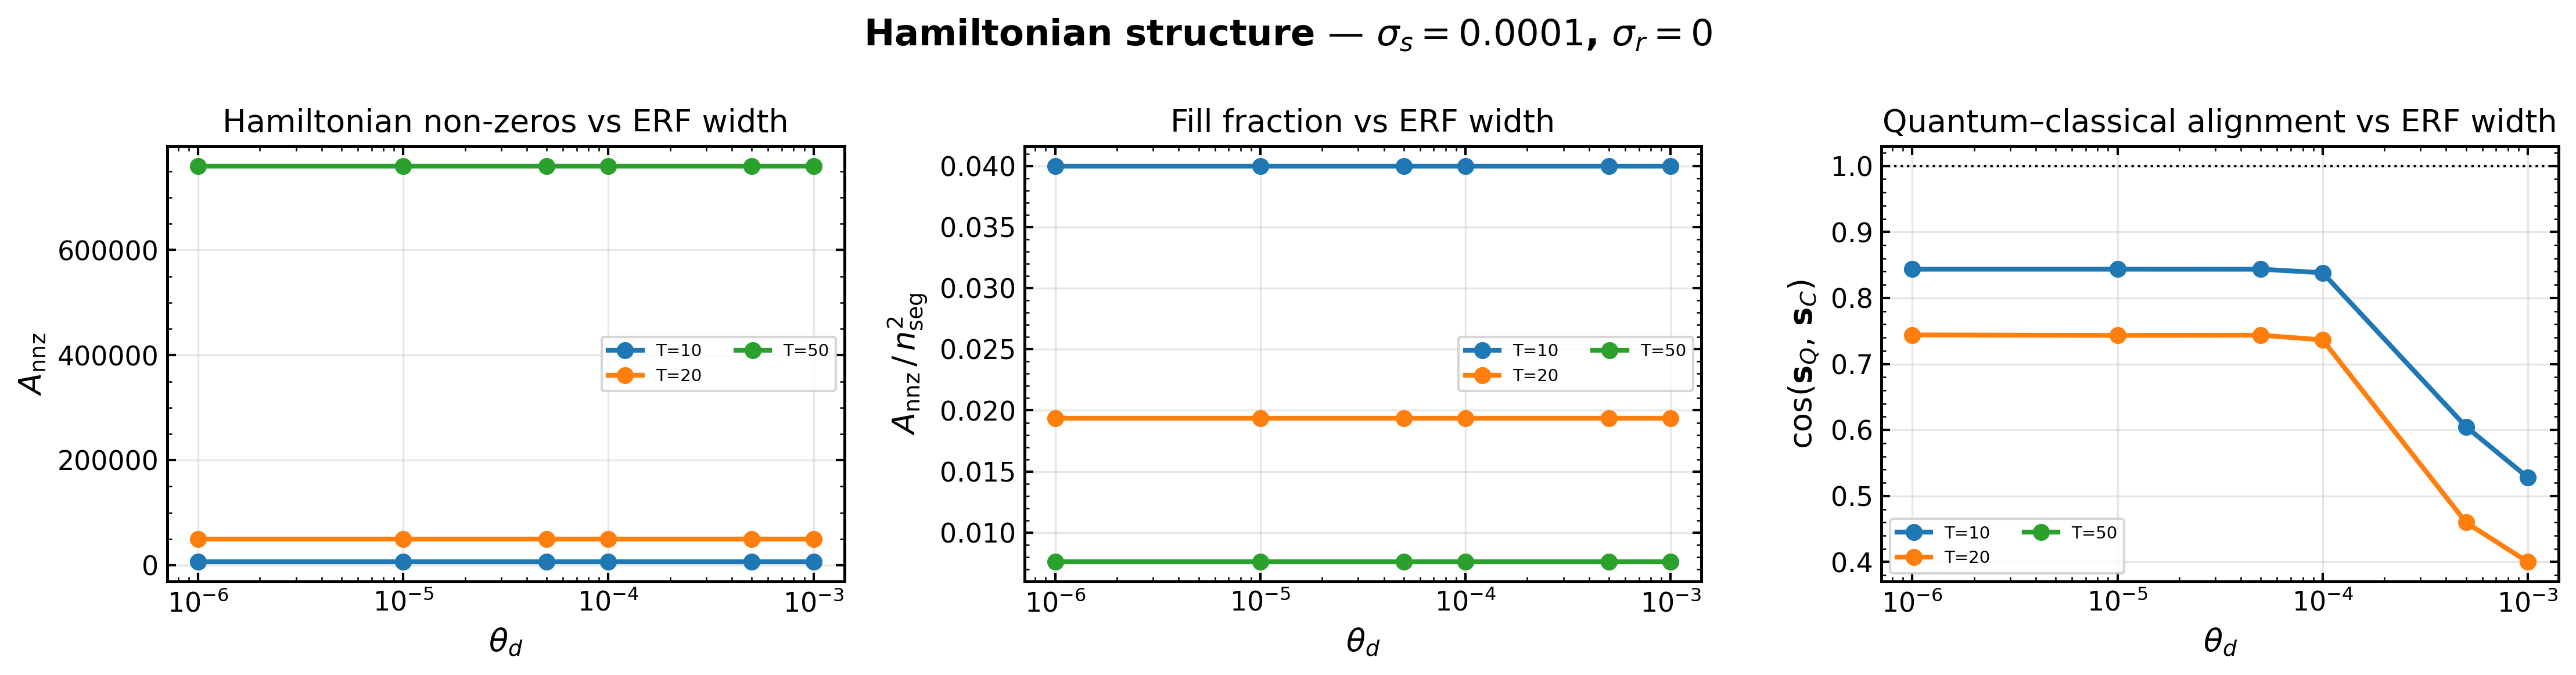
\includegraphics[width=\linewidth]{figures/ham_structure_vs_td.png}
    \caption{Coupling-weight structure vs $\thd$.}
  \end{subfigure}\hfill
  \begin{subfigure}{0.48\linewidth}
    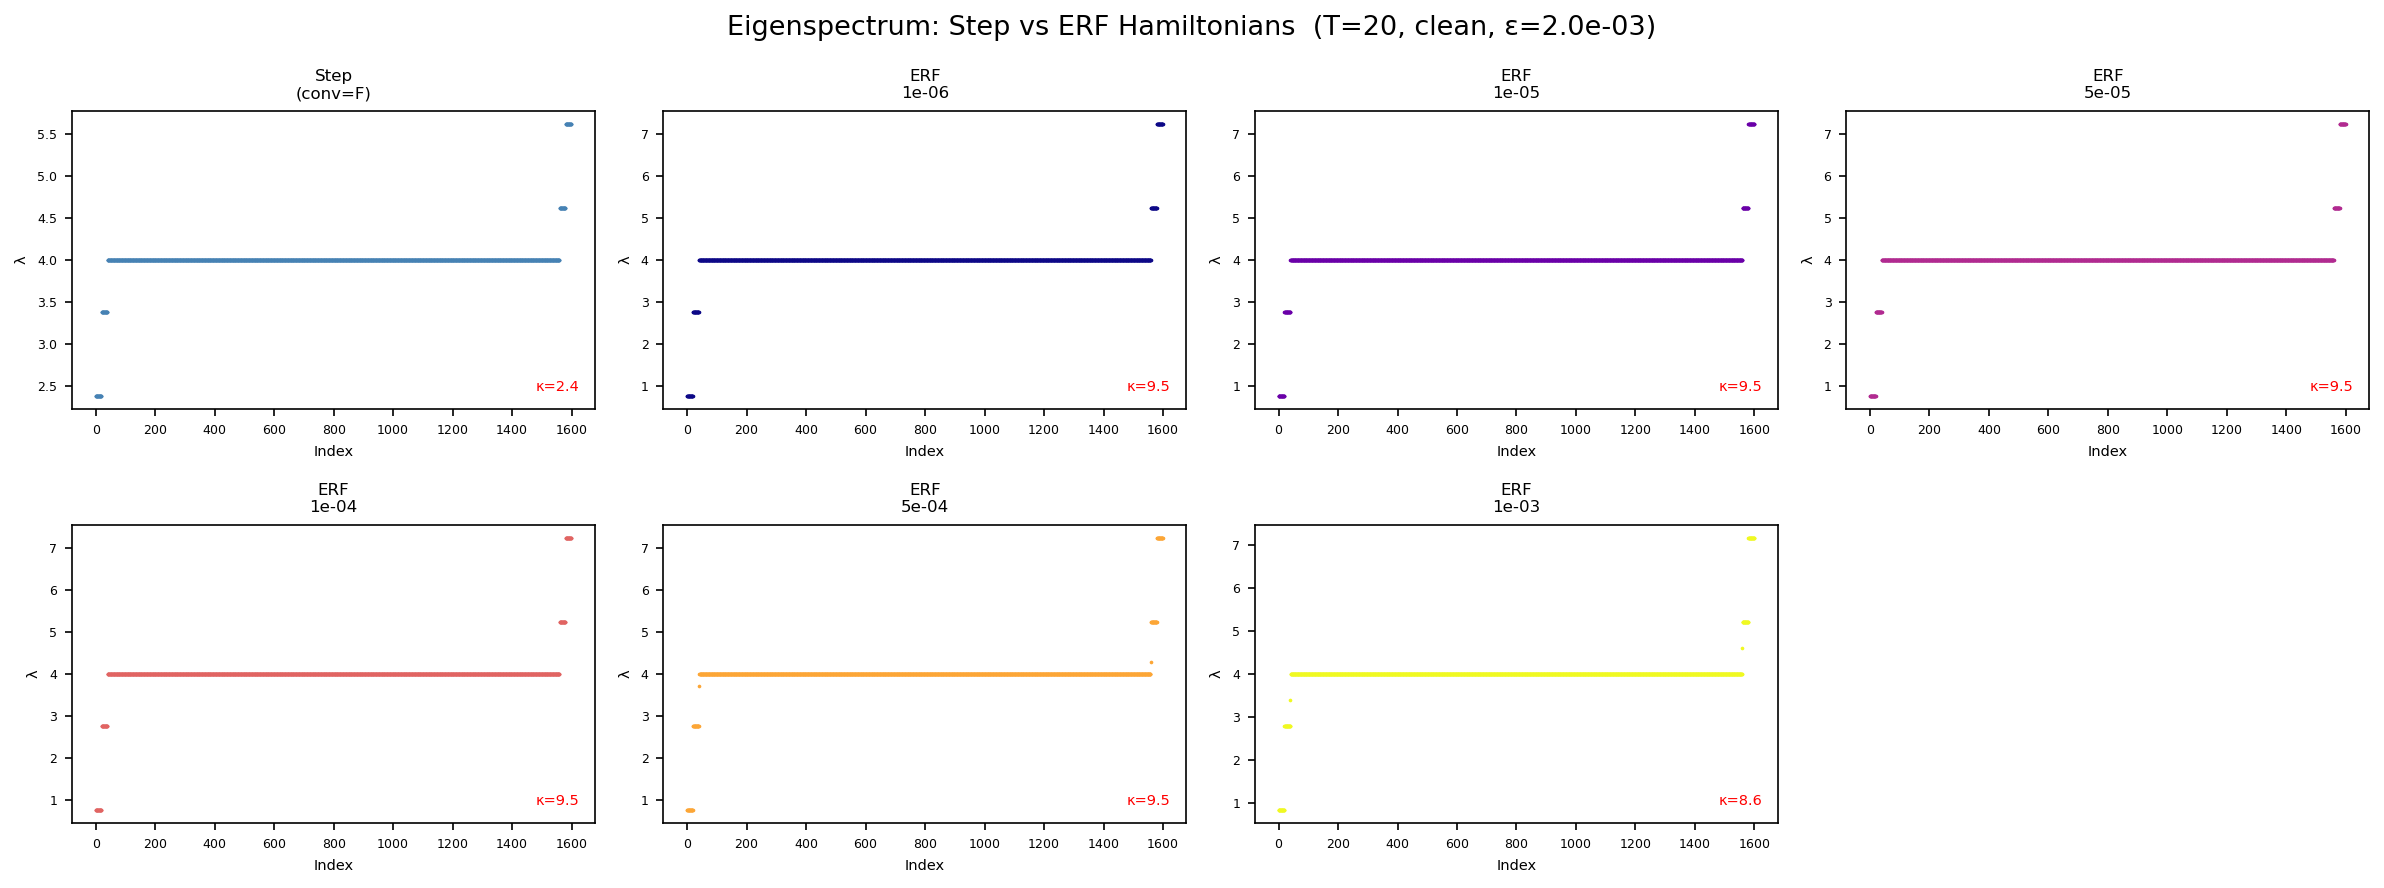
\includegraphics[width=\linewidth]{figures/eigspectrum_step_vs_erf_clean.png}
    \caption{Eigenspectra, step vs \texttt{erf}.}
  \end{subfigure}
  \caption{Structure of the compatibility matrix. The step kernel produces binary
    couplings; the \texttt{erf} kernel spreads weight smoothly across all mid-hit pairs,
    yielding a denser matrix and a compressed eigenspectrum.}
  \label{fig:structure}
\end{figure}

The condition number $\kappa=\lambda_{\max}/\lambda_{\min}$ (Table~\ref{tab:kappa}) is
$\kappa_{\rm step}=2.36$ and $\kappa_{\rm erf}=9.47$ for $\thd\le5\!\times\!10^{-4}$,
falling to $8.55$ at $\thd=10^{-3}$ as the widest kernel weakens the strong true--true
couplings and compresses the spectrum. Crucially $\kappa$ is \emph{unchanged} by the
$1\%$ hit drop (Fig.~\ref{fig:eig_noise}): the spectral shape is a property of $\thd$ and
the geometry, not of the noise realisation.

\begin{table}[H]
  \centering
  \caption{Matrix condition number $\kappa$ at $\ntrk=20$ ($\Nseg=1600$).
    Identical for the clean and $1\%$-drop events.}
  \label{tab:kappa}
  \small
  \begin{tabular}{lccccccc}
    \toprule
    & step & $\thd{=}10^{-6}$ & $10^{-5}$ & $5{\times}10^{-5}$ & $10^{-4}$ & $5{\times}10^{-4}$ & $10^{-3}$ \\
    \midrule
    $\kappa$ & 2.36 & 9.47 & 9.47 & 9.47 & 9.47 & 9.47 & 8.55 \\
    \bottomrule
  \end{tabular}
\end{table}

\begin{figure}[H]
  \centering
  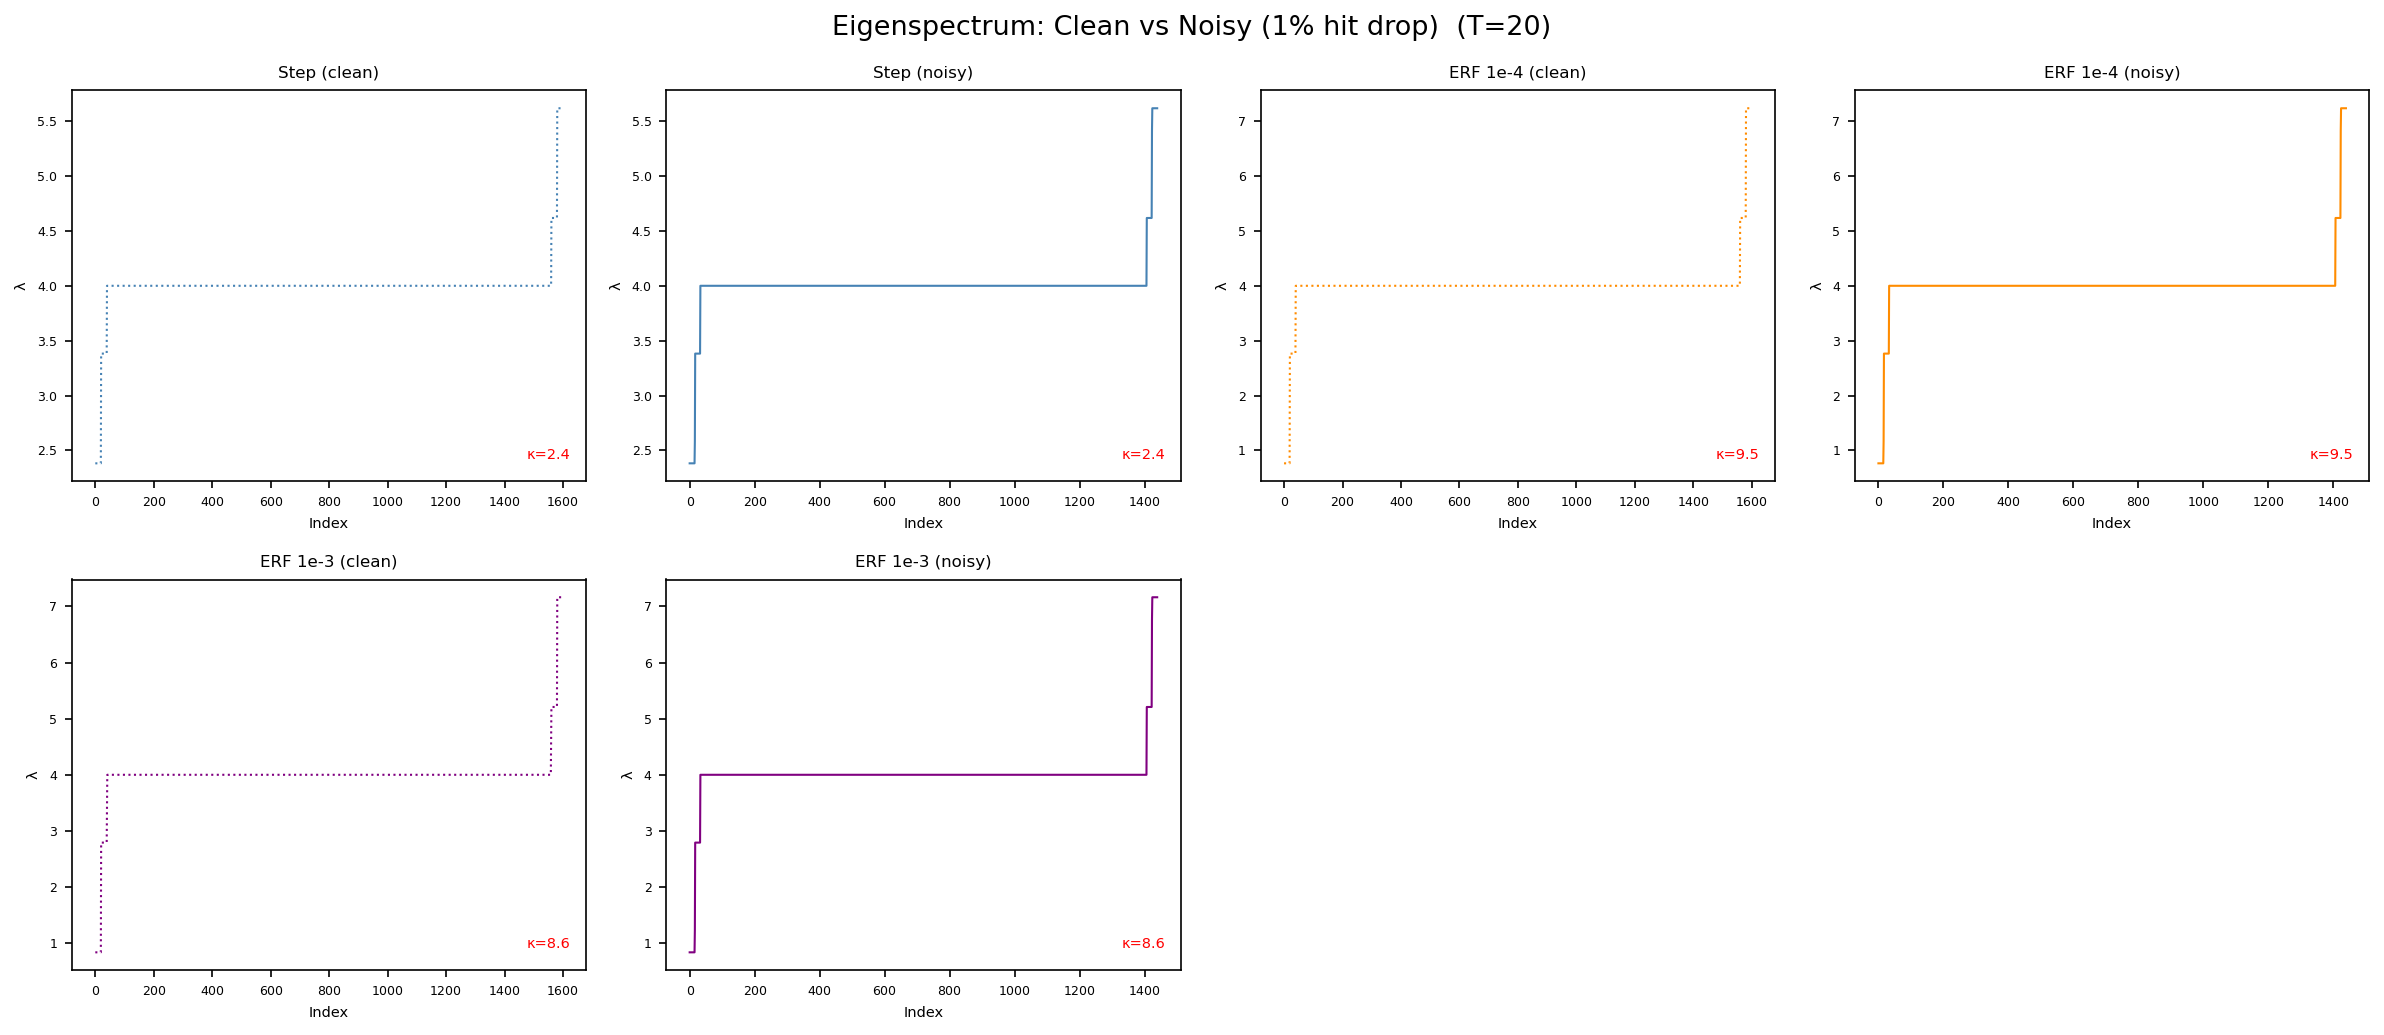
\includegraphics[width=0.7\linewidth]{figures/eigspectrum_noise_delta.png}
  \caption{Eigenspectrum change under $1\%$ hit drop. Both kernels are spectrally
    noise-invariant; $\kappa$ is identical clean vs noisy for every $\thd$.}
  \label{fig:eig_noise}
\end{figure}

\subsection{Classical solution vectors}
\label{sec:results:sol}

\begin{figure}[H]
  \centering
  \begin{subfigure}{0.48\linewidth}
    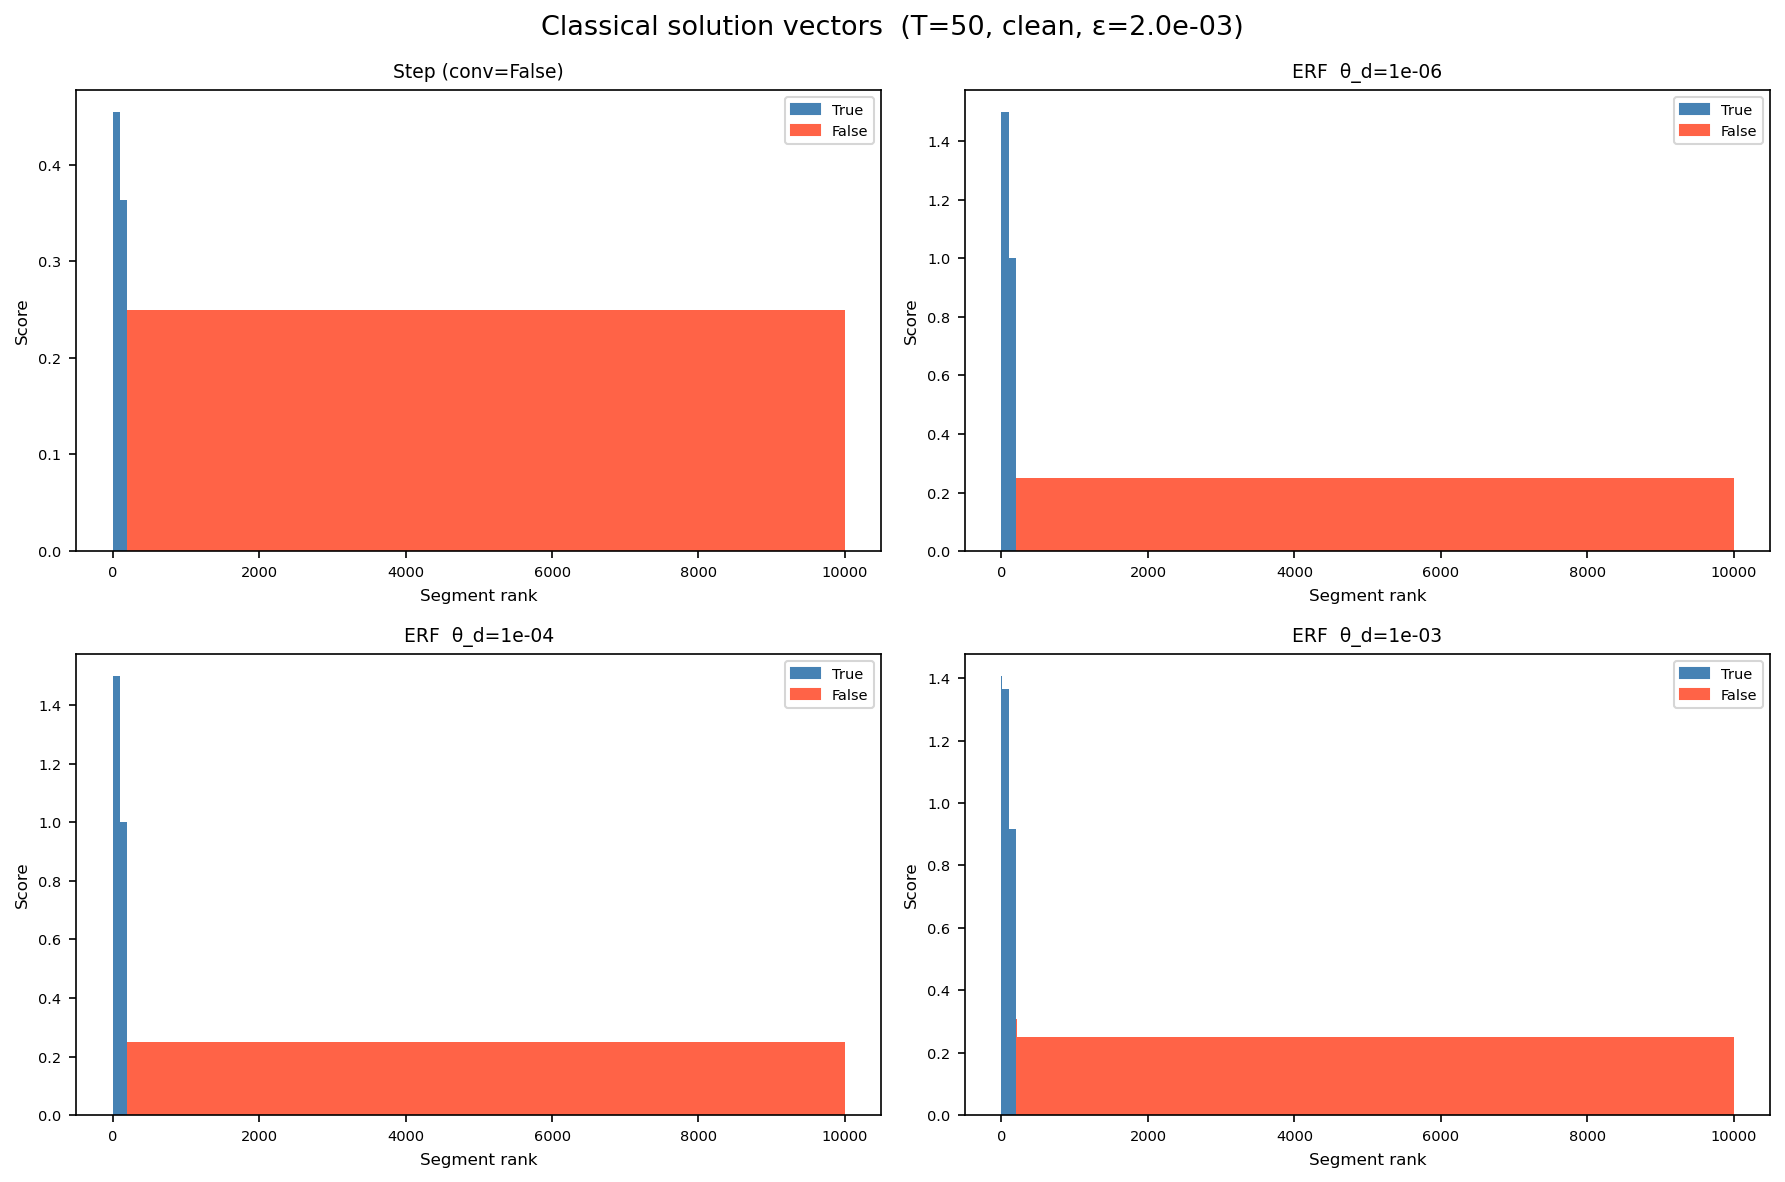
\includegraphics[width=\linewidth]{figures/sol_classical_clean.png}
    \caption{Sorted classical activations.}
  \end{subfigure}\hfill
  \begin{subfigure}{0.48\linewidth}
    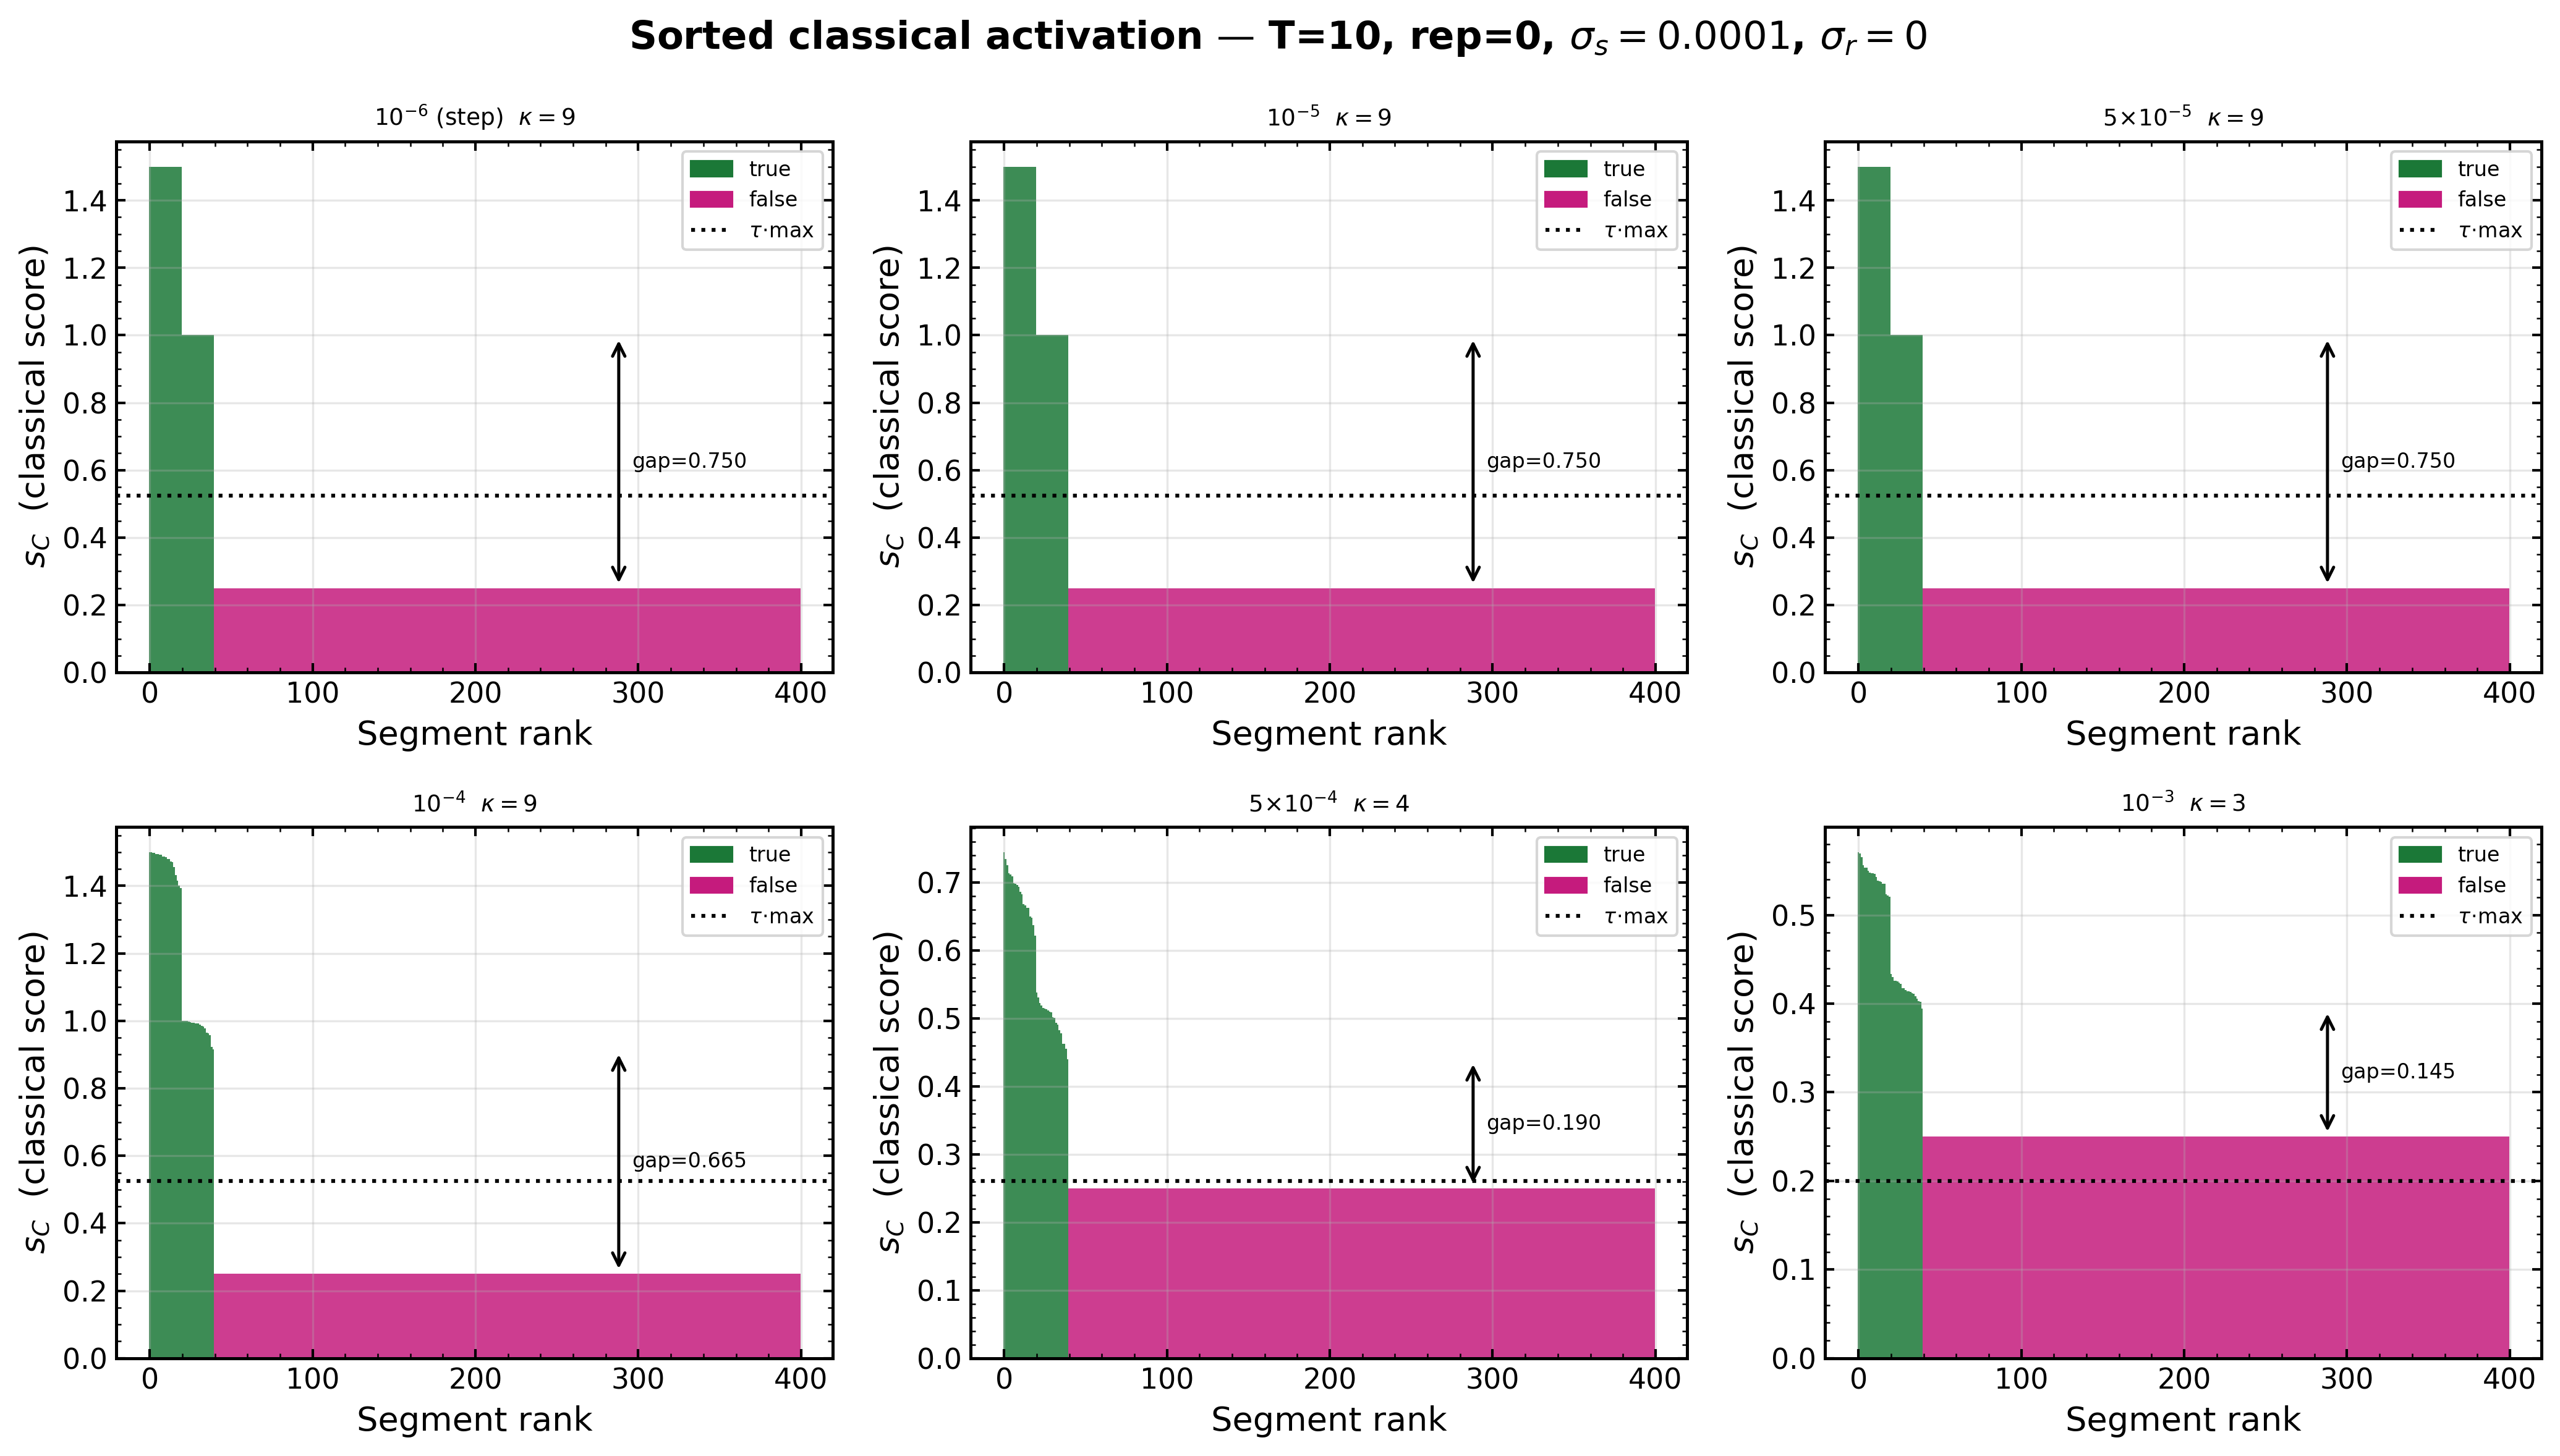
\includegraphics[width=\linewidth]{figures/activation_sorted_T10.png}
    \caption{Activation spectrum, $\ntrk=10$.}
  \end{subfigure}
  \caption{Classical solution vectors. Step-function true segments sit on the $0.375$
    plateau with false segments at the $0.25$ attractor; the \texttt{erf} kernel pushes
    true segments higher (towards $1.0$--$1.5$) but also lifts a few borderline-false
    pairs towards $0.5$.}
  \label{fig:sol}
\end{figure}

Under the step kernel the true activations occupy a narrow $0.36$--$0.45$ band and the
false activations the $0.25$--$0.33$ band, perfectly separated by the $0.35$ threshold.
The \texttt{erf} kernel widens the true band upward (stronger coupling) but, because it
gives partial weight to triplets just outside $\eps$, a small number of false segments
are lifted toward $0.5$ --- the origin of the \texttt{erf} false-rate penalty quantified
below.

\subsection{Segment metrics: clean and noisy}
\label{sec:results:metrics}

\begin{figure}[H]
  \centering
  \begin{subfigure}{0.48\linewidth}
    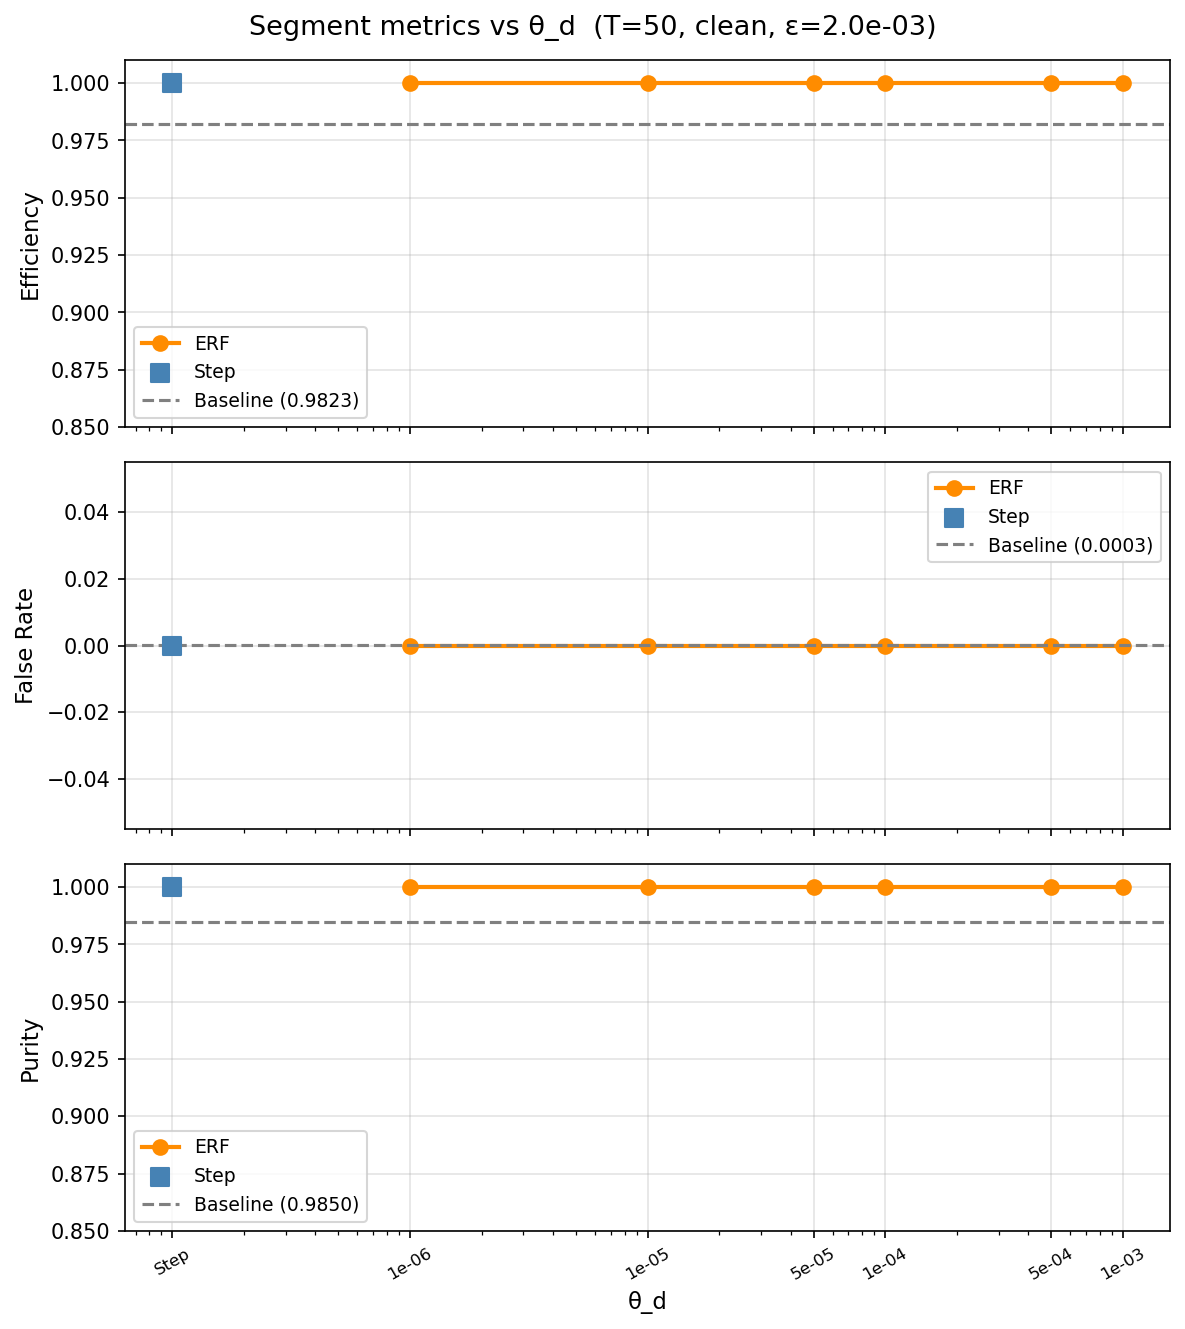
\includegraphics[width=\linewidth]{figures/seg_metrics_clean.png}
    \caption{Clean event.}
  \end{subfigure}\hfill
  \begin{subfigure}{0.48\linewidth}
    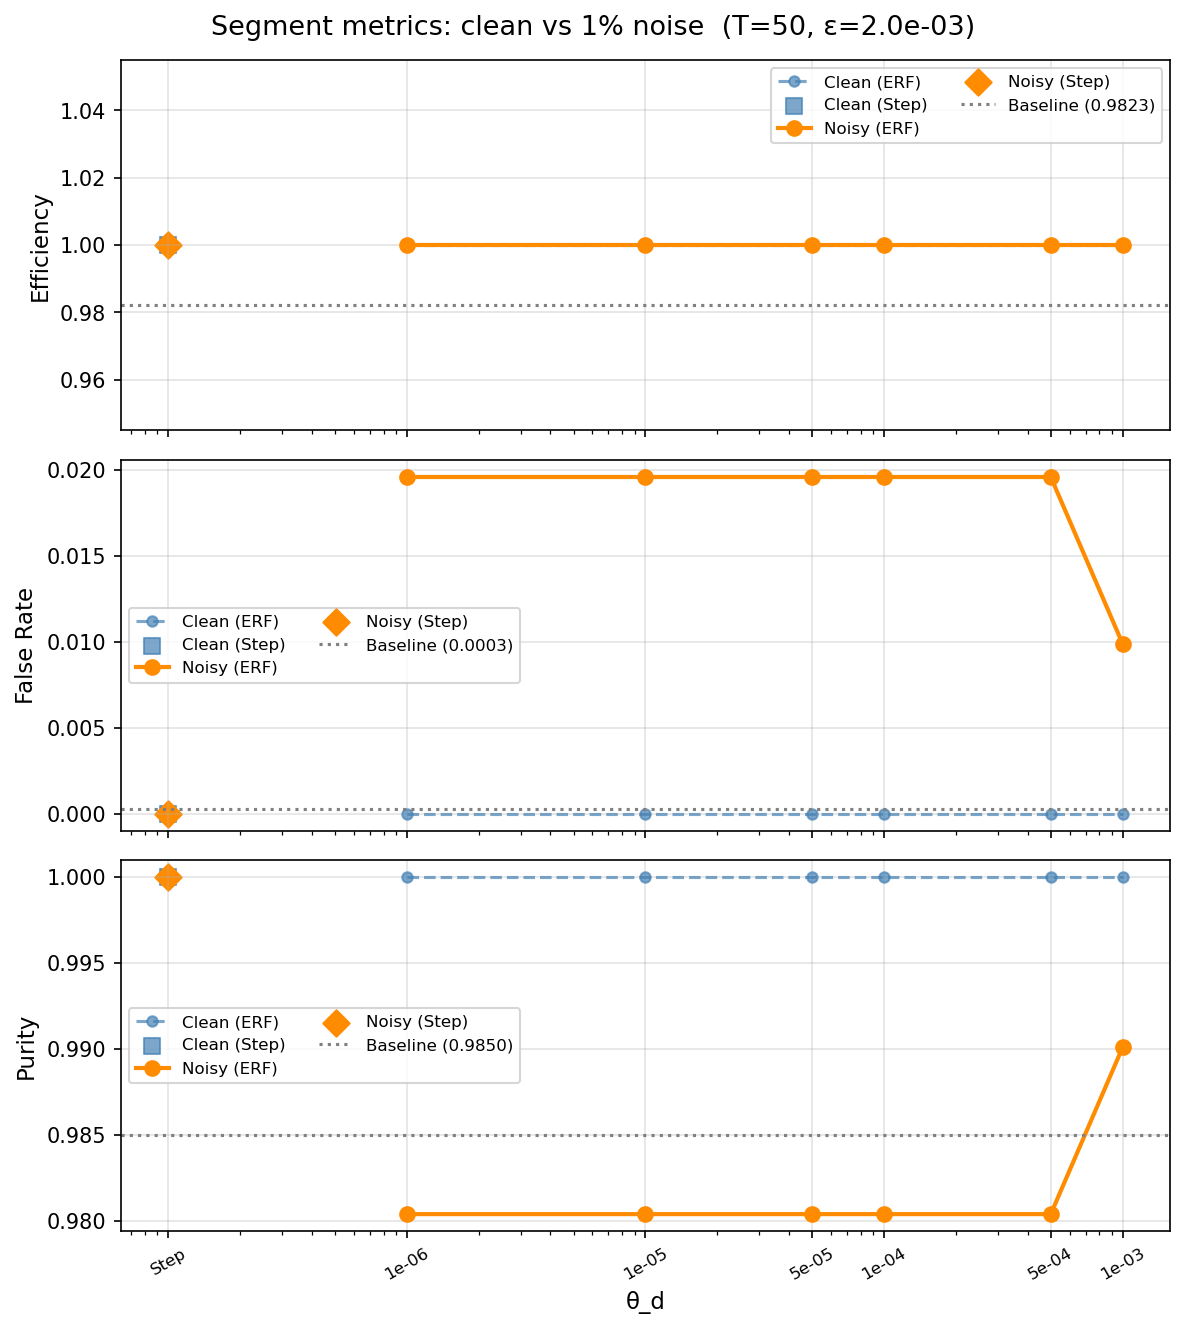
\includegraphics[width=\linewidth]{figures/seg_metrics_noisy.png}
    \caption{$1\%$ hit drop.}
  \end{subfigure}
  \caption{Segment efficiency, false rate and purity vs $\thd$ at $\ntrk=50$, at the
    absolute threshold $x>0.35$. Step shown as the leftmost anchor.}
  \label{fig:seg_metrics}
\end{figure}

On the clean event every kernel achieves efficiency $=1.000$, false rate $=0.000$ and
purity $=1.000$ (Table~\ref{tab:clean}). Under $1\%$ hit drop the step kernel remains
perfect, whereas the \texttt{erf} kernels acquire a small false rate of $0.0196$
($\thd\le5\!\times\!10^{-4}$) or $0.0099$ ($\thd=10^{-3}$), i.e. purity $0.980$--$0.990$.
In other words, in the low-noise regime the simpler step function is at least as good and
carries no false-acceptance cost.

\begin{table}[H]
  \centering
  \caption{Segment metrics at $\ntrk=50$ (threshold $x>0.35$).}
  \label{tab:clean}
  \small
  \begin{tabular}{lccc c ccc}
    \toprule
    & \multicolumn{3}{c}{Clean} & & \multicolumn{3}{c}{$1\%$ hit drop} \\
    \cmidrule(lr){2-4}\cmidrule(lr){6-8}
    Kernel & eff. & false & purity & & eff. & false & purity \\
    \midrule
    step              & 1.000 & 0.000 & 1.000 & & 1.000 & 0.000 & 1.000 \\
    \texttt{erf} $\thd{\le}5{\times}10^{-4}$ & 1.000 & 0.000 & 1.000 & & 1.000 & 0.0196 & 0.980 \\
    \texttt{erf} $\thd{=}10^{-3}$            & 1.000 & 0.000 & 1.000 & & 1.000 & 0.0099 & 0.990 \\
    \bottomrule
  \end{tabular}
\end{table}

\subsection{Resolution scan: where \texttt{erf} wins}
\label{sec:results:scan}

\begin{figure}[H]
  \centering
  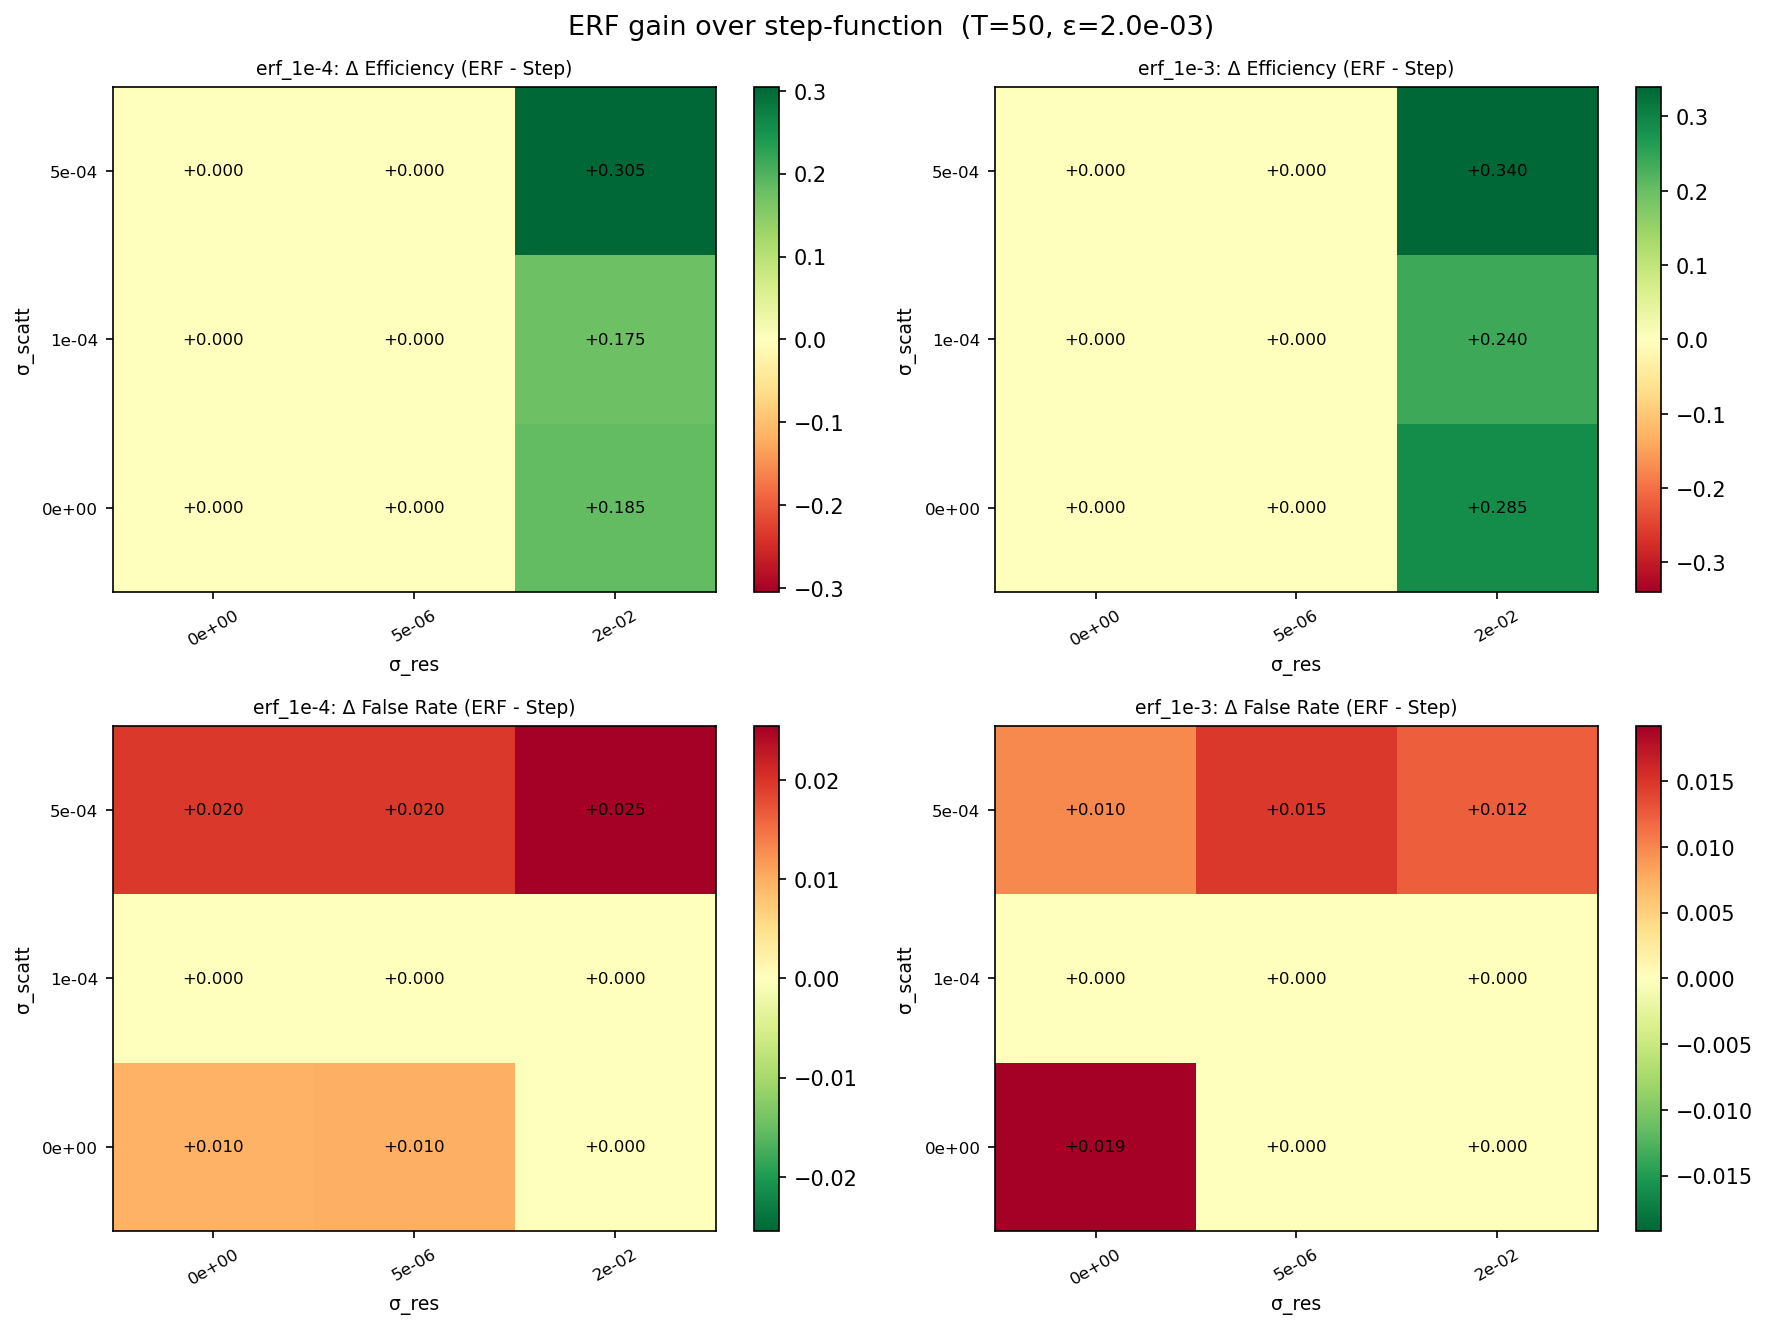
\includegraphics[width=0.92\linewidth]{figures/sigma_scan_delta.png}
  \caption{Segment efficiency vs noise condition for step, \texttt{erf}~$\thd{=}10^{-4}$
    and \texttt{erf}~$\thd{=}10^{-3}$, over the $(\sscat,\sres)$ grid at $\ntrk=50$. The
    \texttt{erf} kernel recovers a large fraction of efficiency at high measurement
    resolution where the step kernel collapses.}
  \label{fig:scan}
\end{figure}

\begin{figure}[H]
  \centering
  \begin{subfigure}{0.32\linewidth}
    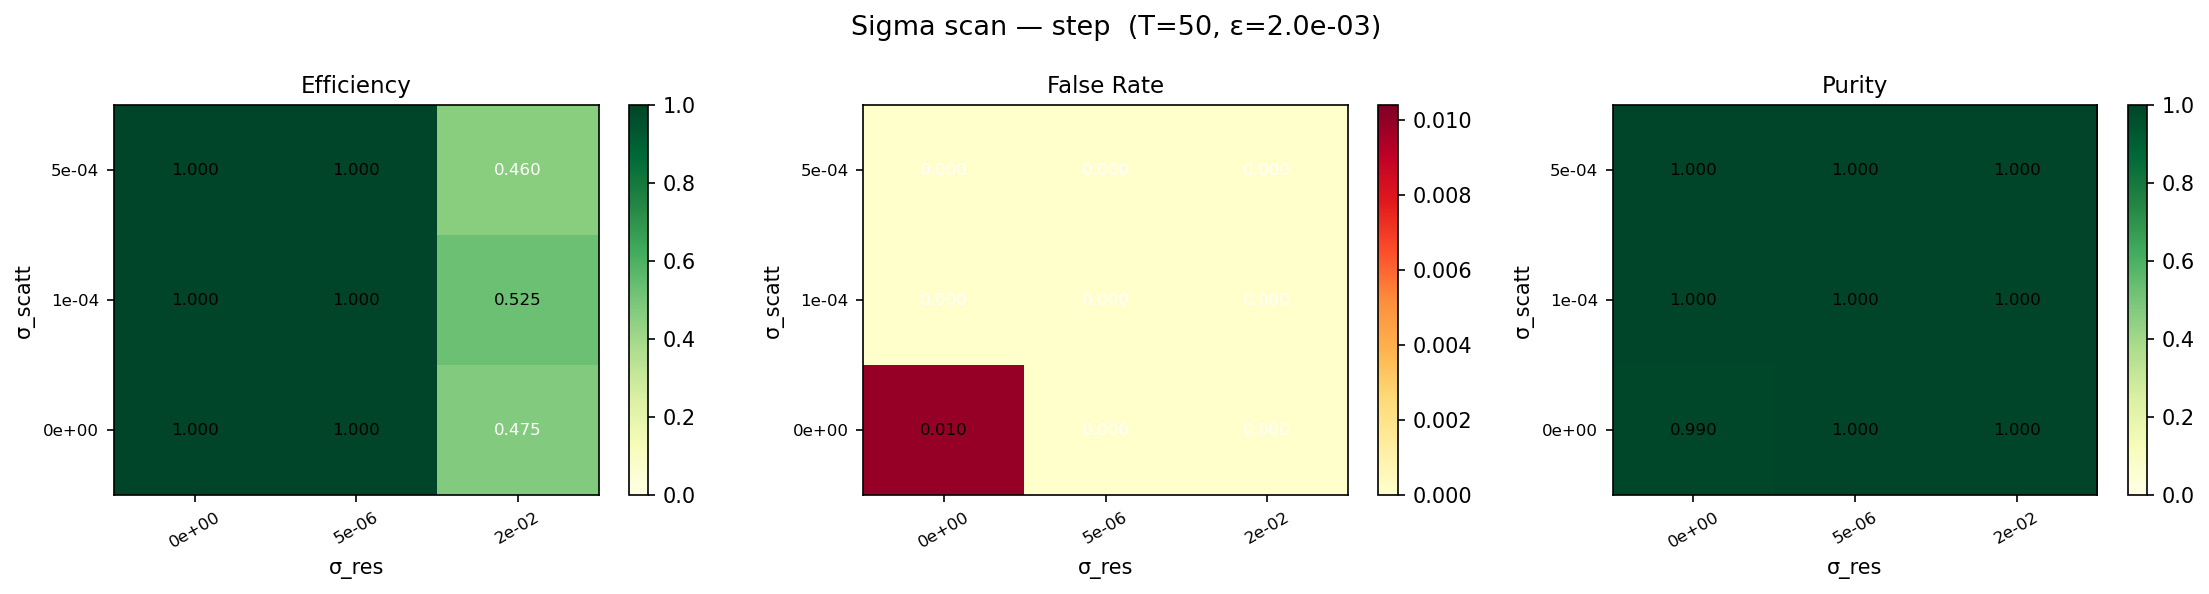
\includegraphics[width=\linewidth]{figures/sigma_scan_heatmap_step.png}
    \caption{step}
  \end{subfigure}\hfill
  \begin{subfigure}{0.32\linewidth}
    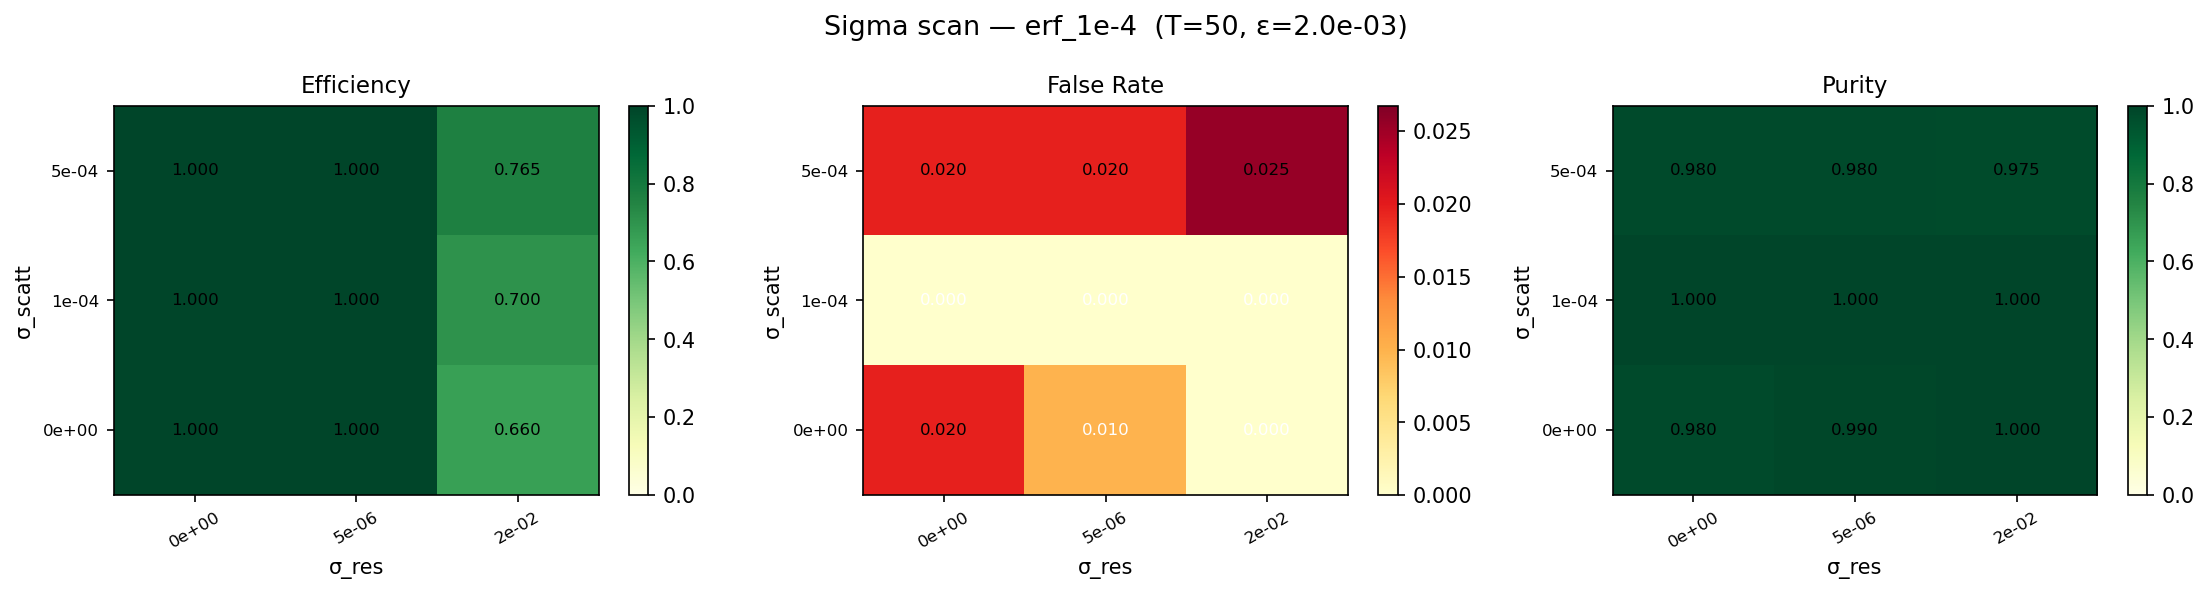
\includegraphics[width=\linewidth]{figures/sigma_scan_heatmap_erf_1e-4.png}
    \caption{\texttt{erf} $\thd{=}10^{-4}$}
  \end{subfigure}\hfill
  \begin{subfigure}{0.32\linewidth}
    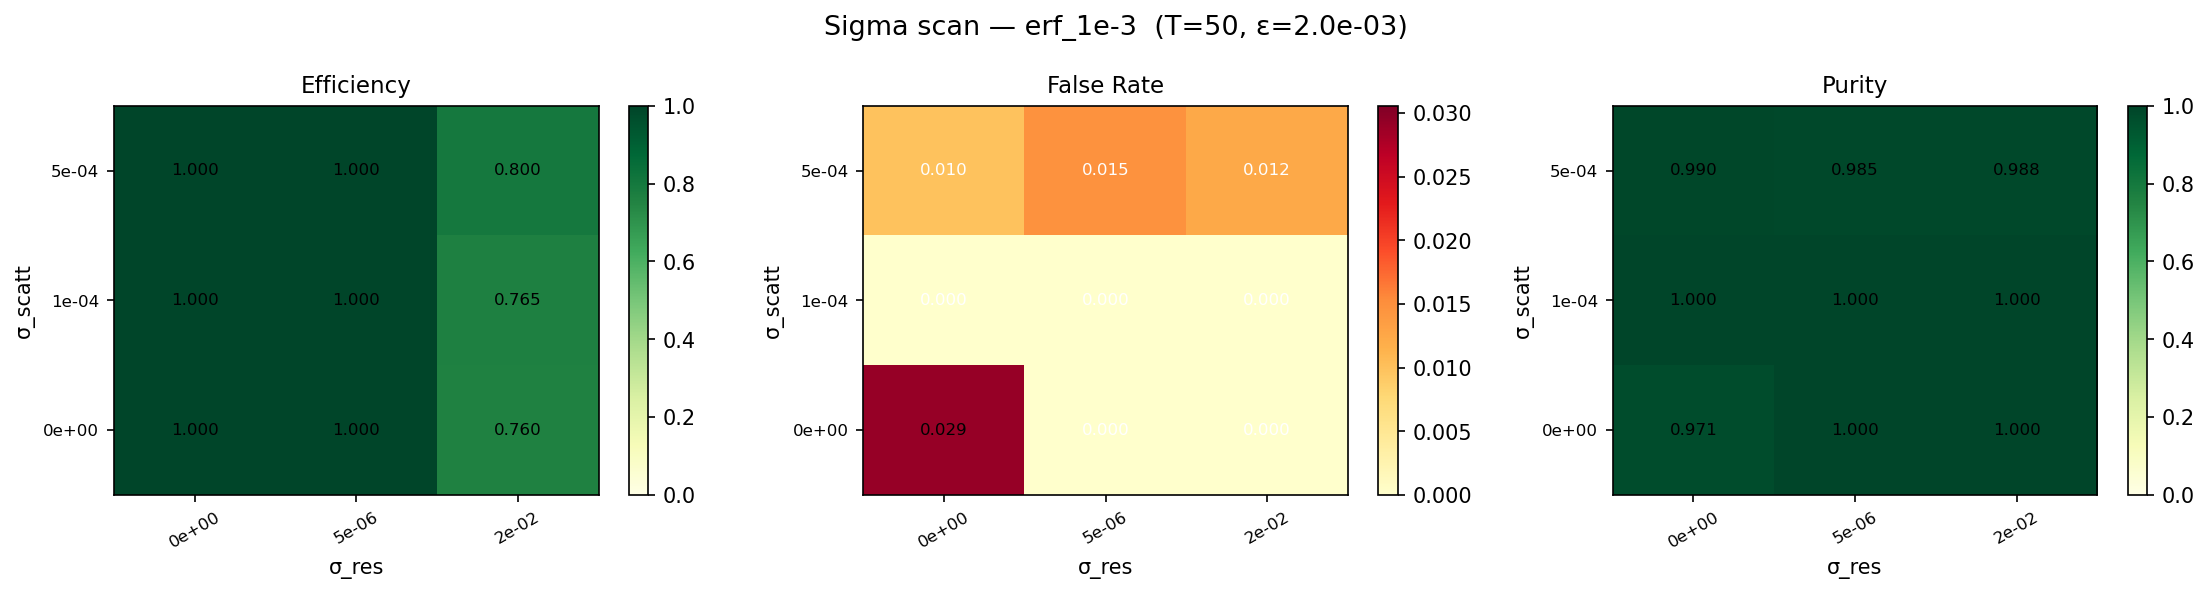
\includegraphics[width=\linewidth]{figures/sigma_scan_heatmap_erf_1e-3.png}
    \caption{\texttt{erf} $\thd{=}10^{-3}$}
  \end{subfigure}
  \caption{Efficiency heatmaps over $(\sscat,\sres)$. The bottom row ($\sres=0.02$)
    is where the kernels diverge.}
  \label{fig:scan_heat}
\end{figure}

The scan (Table~\ref{tab:scan}) isolates the regime where the smooth kernel matters. At
low resolution ($\sres\le5\!\times\!10^{-6}\,\mathrm{mm}$) all kernels give efficiency
$=1.000$ regardless of $\sscat$. At $\sres=0.02\,\mathrm{mm}$ the step efficiency
collapses to $0.46$--$0.53$, because the hard cut rejects true triplets whose kink angle
has been smeared past $\eps$; the \texttt{erf} kernel, which still assigns them partial
weight, recovers efficiency to $0.66$--$0.80$, with the widest kernel
($\thd=10^{-3}$) best at $0.76$--$0.80$. The recovery is $+0.27$ to $+0.34$ in absolute
efficiency, at the cost of a small false rate ($0.012$--$0.026$).

\begin{table}[H]
  \centering
  \caption{Segment efficiency at $\ntrk=50$ across the noise scan (threshold $x>0.35$).
    Only the $\sres=0.02$ rows distinguish the kernels.}
  \label{tab:scan}
  \small
  \begin{tabular}{llccc}
    \toprule
    $\sscat$ & $\sres$ (mm) & step & \texttt{erf} $\thd{=}10^{-4}$ & \texttt{erf} $\thd{=}10^{-3}$ \\
    \midrule
    $0$        & $0.02$ & 0.475 & 0.660 & 0.760 \\
    $10^{-4}$  & $0.02$ & 0.525 & 0.700 & 0.765 \\
    $5\times10^{-4}$ & $0.02$ & 0.460 & 0.765 & 0.800 \\
    \midrule
    \multicolumn{2}{l}{$\sres\le5{\times}10^{-6}$ (any $\sscat$)} & 1.000 & 1.000 & 1.000 \\
    \bottomrule
  \end{tabular}
\end{table}

\subsection{Quantum solution comparison}
\label{sec:results:quantum}

\begin{figure}[H]
  \centering
  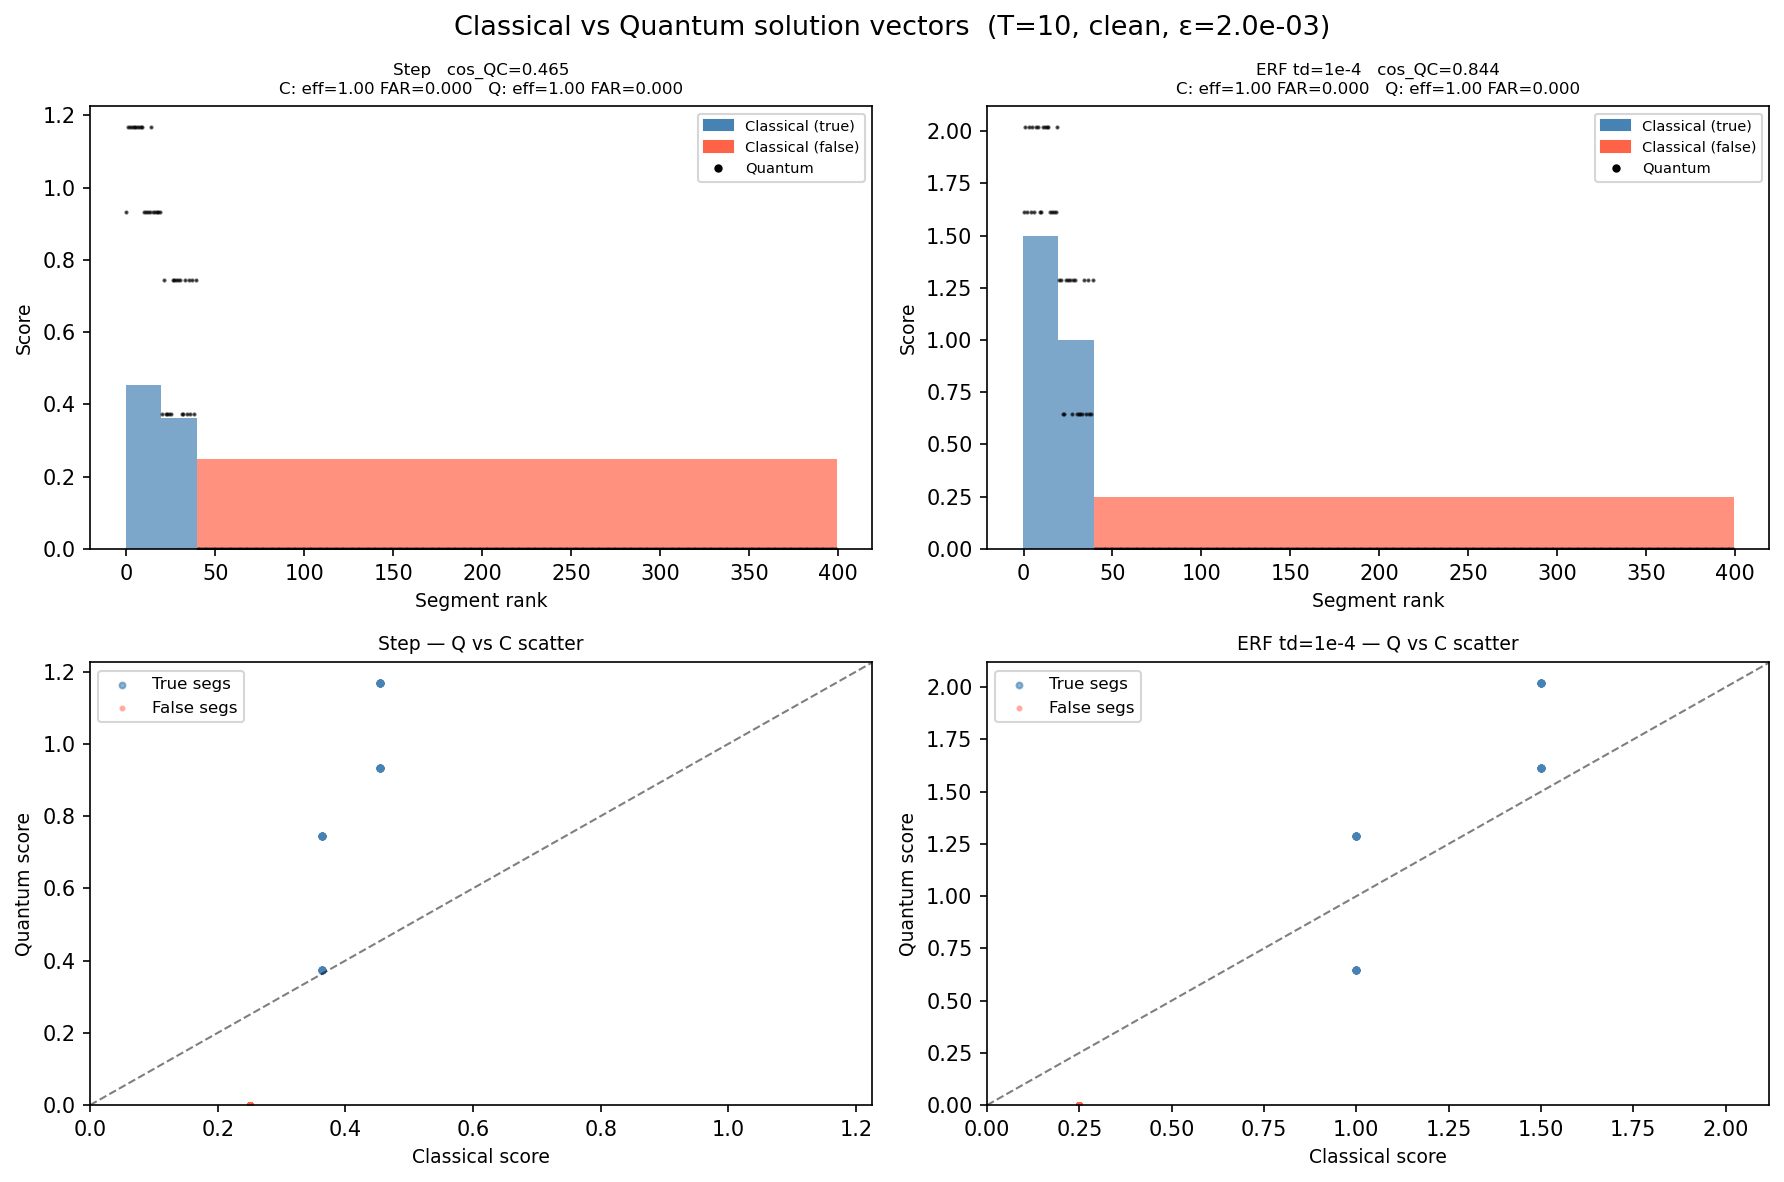
\includegraphics[width=0.92\linewidth]{figures/quantum_comparison_clean_T10.png}
  \caption{Classical vs 1BQF quantum solution vectors at $\ntrk=10$ ($\Nseg=400$,
    9~system qubits), for the step and \texttt{erf}~$\thd{=}10^{-4}$ Hamiltonians.
    Left: sorted classical activations with the quantum solution overlaid; right:
    quantum-vs-classical scatter.}
  \label{fig:quantum}
\end{figure}

Both kernels classify every segment correctly at the absolute threshold (efficiency
$=1.000$, false rate $=0.000$ for classical and quantum alike at $\ntrk=10$). The
\emph{fidelity} of the quantum solution to the classical one, however, differs sharply:
the cosine similarity is $\cosQC=0.465$ for the step kernel but $0.844$ for
\texttt{erf}~$\thd=10^{-4}$, with identical ancilla success probability $P_{\rm anc}=0.0224$.
The smoother \texttt{erf} spectrum aligns the HHL-prepared state with the classical
solution far better, even though its condition number is larger
($\kappa_{\rm erf}=9.5$ vs $\kappa_{\rm step}=2.4$). This is the strongest standalone
argument for the \texttt{erf} kernel.

% ══════════════════════════════════════════════════════════════════════════════
\section{Discussion}
\label{sec:discussion}

\paragraph{When does the \texttt{erf} kernel help?}
The smooth kernel is not a uniform improvement. In low-to-moderate noise the step function
is already perfect at the segment level and the \texttt{erf} kernel only adds a small
false-acceptance penalty by weighting borderline-false pairs. The \texttt{erf} kernel pays
off in exactly one classical regime: large measurement resolution
($\sres\sim0.02\,\mathrm{mm}$), where its tolerance of smeared true triplets recovers
$+0.15$ to $+0.34$ absolute efficiency that the hard cut discards. The widest kernel
tested, $\thd=10^{-3}$, is consistently best for this classical-efficiency recovery.

\paragraph{The condition-number / fidelity puzzle.}
Naively, a smaller condition number should make the quantum (HHL) solution more faithful.
The data show the opposite: the step matrix is better conditioned ($\kappa=2.4$) yet has
the \emph{worse} quantum fidelity ($\cosQC=0.47$), while the \texttt{erf} matrix
($\kappa=9.5$) reaches $\cosQC=0.84$. The resolution is that the 1-bit HHL fidelity is
governed by how well the eigenvalue \emph{distribution} matches the single phase bit, not
by the extremal ratio $\kappa$: the \texttt{erf} kernel's smoother, more clustered
spectrum is better matched by the 1-bit filter. The quantum benefit of \texttt{erf} is
therefore genuine and independent of the classical-efficiency story.

\paragraph{Trade-off summary.}
The \texttt{erf} kernel costs a $74\times$ denser matrix and a small ($\le3\%$)
false-rate penalty in noisy conditions, and buys (i)~classical robustness to resolution
smearing and (ii)~roughly doubled quantum fidelity. Whether the density cost matters at
scale, and whether the fidelity gain persists to higher multiplicities, is the subject of
the in-progress HTCondor sweep.

% ══════════════════════════════════════════════════════════════════════════════
\section{Conclusions}
\label{sec:conclusions}

\begin{enumerate}
  \item \textbf{The step function is the right default at low noise.} With the absolute
        threshold $x>0.35$ it is perfect (efficiency $1.000$, false rate $0.000$); the
        \texttt{erf} kernel matches it but adds a $\le2\%$ false rate under hit drop.
  \item \textbf{\texttt{erf} wins under heavy resolution smearing.} At
        $\sres=0.02\,\mathrm{mm}$ it recovers efficiency from $\sim\!0.5$ (step) to
        $0.76$--$0.80$ ($\thd=10^{-3}$), a $+0.27$ to $+0.34$ absolute gain at a small
        false-rate cost.
  \item \textbf{\texttt{erf} roughly doubles quantum fidelity.} $\cosQC$ rises from
        $0.47$ (step) to $0.84$ (\texttt{erf}, $\thd=10^{-4}$) at $\ntrk=10$, despite a
        larger $\kappa$; the 1-bit HHL filter is matched to the spectral shape, not to
        $\kappa$.
  \item \textbf{The spectrum is noise-invariant.} $\kappa$ depends only on $\thd$
        ($2.4$ step, $8.6$--$9.5$ \texttt{erf}) and is identical clean vs $1\%$-drop.
  \item \textbf{Recommended operating points.} Use the step kernel by default; switch to
        \texttt{erf} $\thd=10^{-3}$ when measurement resolution is large, or
        \texttt{erf} $\thd=10^{-4}$ when running the quantum pipeline.
  \item \textbf{Follow-up (in progress).} The HTCondor sweep
        ($\thd\times(\sscat,\sres)\times\ntrk$, 882 jobs, quantum for $\ntrk\le200$) will
        extend these single-event findings to the full multiplicity landscape and supply
        the Youden-J / EER threshold analysis.
\end{enumerate}

% ── Bibliography ──────────────────────────────────────────────────────────────
\begin{thebibliography}{9}
\bibitem{onebqf}
  X.~Chiotopoulos, D.~Nicotra, G.~Scriven, K.~Driessens, M.~Merk,
  J.~Sch\"{u}tz, J.~de~Vries, M.~H.~M.~Winands,
  \textit{TrackHHL: The 1-Bit Quantum Filter for particle trajectory reconstruction},
  arXiv:2601.07766 [quant-ph] (2026).

\bibitem{hhl}
  A.~W.~Harrow, A.~Hassidim, S.~Lloyd,
  \textit{Quantum Algorithm for Linear Systems of Equations},
  Phys.\ Rev.\ Lett.\ \textbf{103}, 150502 (2009).
\end{thebibliography}

\end{document}
